\section{基于非线性优化方法的状态估计}

继上一节介绍了基于EKF的状态估计方法,本节将继续介绍基于非线性最小二乘的状态估计方法,包括几种主流的求解最小二乘估计的方法以及加速求解的算法,并从理论角度分析滤波法和优化法的优劣。

目前绝大多数的SLAM算法通过集束调整\citep{triggs1999bundle}(Bundle Adjustment)方法来对状态进行估计。在传统的视觉SfM算法中,集束调整是指通过联合优化所有的视觉观测误差来同时求解最优的相机位姿状态和三维点状态的方法。而对于使用了更多传感器的SLAM系统,除了三维点和位姿状态,集束调整算法还需要实时地、持续对系统的其他状态比作出估计。对于VISLAM,集束调整通常会通过联合优化所有的视觉观测和惯性观测来同时求解相机或IMU的位姿、速度以及IMU的bias状态。

\subsection{基于图优化的状态估计}

图优化方法是分析并求解SLAM后端状态估计问题的常用工具。最早在机器人领域,为了解决多段激光传感器数据额融合时的全局一致性问题,\citep{lu1997globally,lu1997robot}提出了基于位姿图的优化方法。\citep{thrun2006graph}在此基础上进一步提出了GraphSLAM,使用由位姿状态和三维点状态以及它们之间的约束构成的因子图来描述集束调整问题。因子图可以很直观地描述集束调整问题中状态和约束之间的关联,有助于分析集束调整问题的各种性质。经过长时间的发展,图优化方法已经成为SLAM领域的经典方法。

\begin{figure}[htb!]
    \centering
    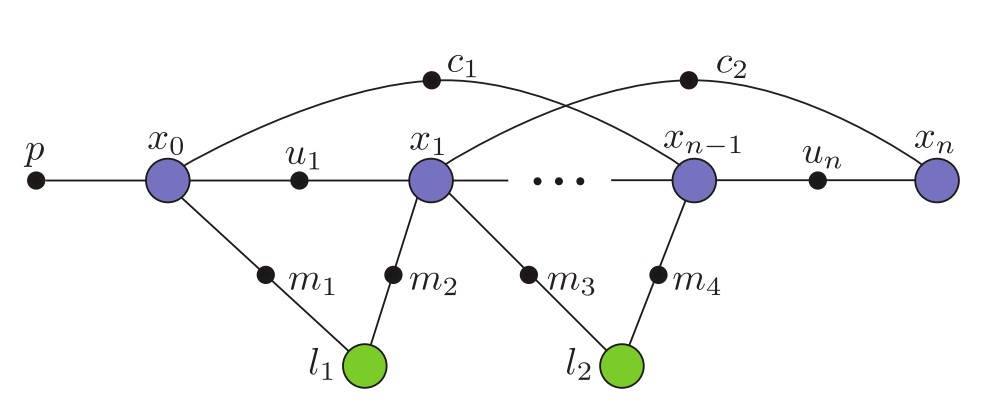
\includegraphics[width=.6\textwidth]{Pictures/isam_factor_graph.png}
    \caption{因子图示例\citep{kaess2012isam2}:紫色节点代表位姿状态,绿色节点代表三维点状态,黑色节点代表状态之间的约束因子。}
    \label{fig:isam_factor_graph}
\end{figure}

图~\ref{fig:isam_factor_graph}展示了一类常见的因子图结构。按照图示的例子,一个SLAM问题中可能存在的约束有状态变量的先验约束$p$,相邻状态之间的相对位姿约束$u_1 \dots u_n$,非相邻状态之间的回路闭合约束$c_1,c_2$以及视觉观测约束$m_1 \dots m_4$等。而求解完整集束调整的过程就相当于最大化整个因子图中的所有约束的集合$\mathcal{Z}$关于所有状态集合$\mathcal{X}$的联合条件概率:
\begin{equation}
    P(\mathcal{Z}|\mathcal{X}) = \prod_{f_i\in\mathcal{Z}} P(f_i(\mathcal{X}_i))
\end{equation}
其中$\mathcal{X}_i$代表所有与约束节点$f_i$相邻的状态节点。通常会假设这是一个高度非线性系统,并且所有的约束$f_i$的噪声服从高斯分布$f_i\sim\mathcal{N}(\mu_i, \sigma_i^2)$。这样的的概率最大化问题通常被转化为非线性最小二乘问题来求解:
\begin{equation}
\begin{aligned}
    \mathcal{X}^\star &= \mathop{\arg\max}_{\mathcal{X}}
                         \prod_{f_i\in\mathcal{Z}} P(f_i(\mathcal{X}_i)) \\
                      &= \mathop{\arg\min}_{\mathcal{X}}
                         \sum_{f_i\in\mathcal{Z}} \tfrac{1}{2}
                         \left\| f_i(\mathcal{X}_i)) \right\|_{\sigma_i^2}^2
\end{aligned}
\end{equation}

\subsection{非线性最小二乘}

非线性最小二乘问题难以被直接求解,通常要使用迭代求解的方法来逼近局部最优解。如果变量的初值在全局最优解的附近,则一般可以使用牛顿法(Newton's method)迭代求解。如下给出了而一个典型的非线性最小二乘问题$F(\bm{x})$的形式:
\begin{equation}
    F(\bm{x}) = \tfrac{1}{2} \Vert \bm{f}(\bm{x}) \Vert^2
\label{eq:nls}
\end{equation}
其中变量$\bm{x}\in\mathbb{R}^n$,$\bm{f}(\cdot):\mathbb{R}^n\mapsto\mathbb{R}^m$为关于变量$\bm{x}$的非线性代价函数,即目标函数。在局部最优解附近,最小化能量函数$F(\cdot)$:
\begin{equation}
    \bm{x}^\star = \mathop{\arg\min}_{\bm{x}} F(\bm{x})
\end{equation}
等同于求解其梯度函数$\bm{g}(\cdot)$的零点(对于线性的函数则为唯一的零点),即:
\begin{equation}
    \bm{g}(\bm{x}) = \nabla F(\bm{x}) = \begin{bmatrix}
        \frac{\partial F}{\partial x_1} &
        \frac{\partial F}{\partial x_2} &
        \cdots &
        \frac{\partial F}{\partial x_n}
    \end{bmatrix}^\top = \bm{0}
\end{equation}
采用牛顿法求解上述零点问题,记梯度函数$\bm{g}(\cdot)$的一阶导数为海森矩阵(Hessian matrix):
\begin{equation}
    \mathrm{H} = \begin{bmatrix}
        \frac{\partial^2 F}{\partial x_1^2} &
        \frac{\partial^2 F}{\partial x_1 \partial x_2} &
        \cdots & \cdots &
        \frac{\partial^2 F}{\partial x_1 \partial x_n} \\
        %
        \frac{\partial^2 F}{\partial x_2 \partial x_1} &
        \frac{\partial^2 F}{\partial x_2^2} &
        & &
        \frac{\partial^2 F}{\partial x_2 \partial x_n} \\
        %
        \vdots & & \ddots & & \vdots \\
        \vdots & & & \ddots & \vdots \\
        %
        \frac{\partial^2 F}{\partial x_n \partial x_1} &
        \frac{\partial^2 F}{\partial x_n \partial x_2} &
        \cdots & \cdots &
        \frac{\partial^2 F}{\partial x_n^2}
    \end{bmatrix}
\end{equation}
求解如下线性系统:
\begin{equation}
    \bm{\delta} = \mathrm{H} \:\setminus\: \bm{\eta}
    \label{eq:linsys}
\end{equation}
其中$\bm{\eta}=-\bm{g}(\bm{x})$。使用$\bm{\delta}$更新变量:$\bm{x}\leftarrow\bm{x}+\bm{\delta}$。 式\eqref{eq:linsys}通常称为正规方程(normal equation),如上求解非线性最小二乘的方法则为正规方程法。线性的问题中,矩阵$\mathrm{H}(\bm{x})$至少为半正定矩阵, 给定任意初值$\bm{x}$(这里选择了初值为$\bm{0}$)只需一步就可解得 式\eqref{eq:nls}的全局最优解。而对于非线性的情况,则需要多次迭代才能解得局部最优解。

\subsection{高斯-牛顿法}\label{sec:gn}

对于非线性最小二乘问题,牛顿法中计算函数$F(\cdot)$的准确海森矩阵$\mathrm{H}$的代价往往很大,甚至没有闭解。一些算法会寻求使用近似方法计算每次迭代的海森矩阵,比如拟牛顿法\citep{tingleff2004methods}(Qausi-Newton method)。拟牛顿法适用于一般的最小化问题,而对于非线性最小二乘问题,通常可以高斯-牛顿法(Gauss-Newton method)求解。高斯-牛顿法是用于求解非线性最小二乘问题的经典迭代算法,也是众多其他迭代算法的基础。

依然考虑非线性最小二乘问题\eqref{eq:nls},使用高斯-牛顿法迭代求解,首先要给定变量的初值$\bm{x}=\bm{x}_0$。对其在当前点处进行泰勒展开,并忽略高阶项,可得目标函数$\bm{f}(\cdot)$在$\bm{x}$处的线性近似:
\begin{equation}
    \bm{f}(\bm{x}+\bm{\delta}) \simeq \bm{f}(\bm{x}) + \mathrm{J}\bm{\delta}
\end{equation}
其中$\mathrm{J}\in\mathbb{R}^{m \times n}$是目标函数$\bm{f}(\cdot)$在$\bm{x}$处的雅各比矩阵(Jacobian)。相应地,
\begin{equation}
\begin{aligned}
    F(\bm{x}+\bm{\delta}) \simeq L(\bm{\delta})
        &= \tfrac{1}{2} \Vert \bm{f}(\bm{x}) + \mathrm{J}\bm{\delta} \Vert^2 \\
        &= F(\bm{x}) + \mathrm{J}^\top\bm{f} +
           \tfrac{1}{2}\bm{\delta}^\top\mathrm{J}^\top\mathrm{J}\bm{\delta}
\end{aligned}
\label{eq:linmod}
\end{equation}
 式\eqref{eq:nls}被转化为局部$\bm{x}$处的线性最小二乘子问题,使用牛顿法求解这个线性最小二乘子问题
\begin{equation}
    \min_{\bm{\delta}} \tfrac{1}{2}
    \Vert \bm{f}(\bm{x}) + \mathrm{J}\bm{\delta} \Vert^2
    \label{eq:lls}
\end{equation}
需要构建正规方程:
\begin{equation}
    \mathrm{H}_{gn} = \mathrm{J}^\top\mathrm{J}, \quad
    \bm{\eta}       = -\mathrm{J}^\top\bm{f}(\bm{x})
    \label{eq:normal_eq}
\end{equation}
再求解,得到高斯-牛顿法一次迭代的结果:
\begin{equation}
    \bm{\delta}_{gn} = \mathrm{H}_{gn} \:\setminus\: \bm{\eta}
    \label{eq:gn}
\end{equation}
将此结果更新至变量:$\bm{x}\leftarrow\bm{x}+\bm{\delta}$,然后不断重复以上过程,直至结果收敛。

 式\eqref{eq:normal_eq}和\eqref{eq:linsys}的形式类似,也可以认为高斯-牛顿法和牛顿法的最大区别就是高斯-牛顿法使用了$\mathrm{J}^\top\mathrm{J}$来近似海森矩阵。

\subsection{莱文贝格-马夸特方法}

除了高斯-牛顿法之外,还有一种经典的求解非线性最小二乘优化的算法:莱文贝格-马夸特(Levenberg-Marquardt)法。它也被认为是带有阻尼因子的高斯-牛顿法,也是信赖域方法(trust region method)的前身\citep{jorge2006numerical}。

前面提到,一般的纯视觉的SLAM算法中,尺度是不可观测的,也就是说VSLAM的状态估计中,对全局所有的三维点坐标和相机位置进行统一的缩放,不会引起重投影误差的改变(在不考虑数值误差的情况下)。从求解VSLAM集束调整问题的角度来看,这一性质造成了在直接使用高斯-牛顿法时海森矩阵的秩亏现象,即矩阵$\mathrm{J}^\top\mathrm{J}$为半正定的情况。此时直接使用矩阵分解求逆的方法求解线性最小二乘子问题就会得到数值不稳定的结果,比如解得的步长在某个方向过大等。

\subsubsection*{莱文贝格法}

针对这一情况,莱文贝格在基础的高斯-牛顿法中引入了对迭代步长的直接约束,将原先每次迭代的线性最小二乘子问题改写为:
\begin{equation}
    \mathop{\min}_{\bm{\delta}} \tfrac{1}{2}
    \left(
        \Vert \bm{f}(\bm{x}) + \mathrm{J}\bm{\delta} \Vert^2 +
        \mu \Vert \bm{\delta} \Vert^2
    \right), \quad \mu > 0
\end{equation}
这样一来,原先高斯-牛顿法求解的正规方程就变成了
\begin{equation}
    \mathrm{H}_{l} = \left( \mathrm{J}^\top\mathrm{J}+\mu\mathrm{I} \right), \quad
    \bm{\eta}      = -\mathrm{J}^\top\bm{f}(\bm{x})
\end{equation}
\begin{equation}
    \bm{\delta}_{l} = \mathrm{H}_{l} \:\setminus\: \bm{\eta}
    \label{eq:levenberg}
\end{equation}
其中的$\mu$就是所谓的阻尼因子(damping factor)。

阻尼因子控制住了每次迭代计算的步长的模。通常阻尼因子$\mu$具备下面三个性质\citep{tingleff2004methods}:
\begin{enumerate}
    \item 对于任意的$\mu>0$,海森矩阵$(\mathrm{J}^\top\mathrm{J}+\mu\mathrm{I})$正定,这一点保证了求得的步长$\bm{\delta}$处于能量下降的方向;
    \item 当$\mu\to\infty$时,求得的步长$\bm{\delta}$接近于最速下降方向$-\frac{1}{\mu}\mathrm{J}^\top\bm{f}(\bm{x})$,当当前的变量$\bm{x}$ 的值距离最优解较远时,最速下降的方向更容易符合预期;
    \item 当$\mu\to0$时,则求得的步长$\bm{\delta}$更接近于高斯-牛顿法的结果,如果当前变量$\bm{x}$的值较为接近最优解,则这样的步长更容易符合预期,因为在收敛点附近,真实的海森矩阵更接近标准的二次型形式。
\end{enumerate}
同时,由于正则项$\mu\mathrm{I}$的加入,修改后的海森矩阵$(\mathrm{J}^\top\mathrm{J}+\mu\mathrm{I})$一定为正定二次型矩阵,提升了求解的数值稳定性。

\subsubsection*{莱文贝格-马夸特法}

莱文贝格在海森矩阵的每一个主元上都施加了同样的阻尼限制$\mu$,某种程度上将是对步长$\bm{\delta}$在各个梯度方向上施加了相同的限制,这显然不是最合理的做法。当$\mu$非常大的时候,一定程度上由原始海森矩阵$\mathrm{J}^\top\mathrm{J}$提供的信息就被抑制了,难以被利用。马夸特在莱文贝格的方法上进行了改进,根据海森矩阵的主元大小,对步长的不同梯度方向施加不同的阻尼:
\begin{equation}
    \mathrm{H} = \left( \mathrm{J}^\top\mathrm{J}+\mu\mathbf{diag}(\mathrm{J}^\top\mathrm{J}) \right), \quad
    \bm{\eta}  = -\mathrm{J}^\top\bm{f}(\bm{x})
\end{equation}
\begin{equation}
    \bm{\delta}_{lm} = \mathrm{H} \:\setminus\: \bm{\eta}
    \label{eq:lm}
\end{equation}
这样一来,在梯度较小的方向阻尼较小,$\bm{\delta}_{lm}$的分量也就较大,反之则阻尼较大,$\bm{\delta}_{lm}$的分量较小。得益于更合理的阻尼设置,相对于单纯的莱文贝格法,莱文贝格-马夸特方法在实际应用中的收敛效率要更好。

\subsection{Dog-Leg法}

Dog-Leg法是另一个经典的求解非线性最小二乘优化的算法,也是信赖域方法的代表。莱文贝格-马夸特方法通过阻尼因子来间接地控制每一次迭代的步长,而Dog-Leg法则显式地使用了信赖域来约束每一次迭代的步长。下面给出传统的使用Dog-Leg法求解问题\eqref{eq:nls}的步骤\citep{tingleff2004methods}。首先按照常规的求解步骤进行线性化,得到线性最小二乘子问题\eqref{eq:lls}。Dog-Leg法首先使用 式\eqref{eq:gn}求解高斯-牛顿迭代步$\bm{\delta}_{gn}$,然后使用最速下降法求解一阶迭代步:
\begin{equation}
    \bm{\delta}_{sd} = -\frac{\left\|\bm{g}\right\|^2}
                             {\left\|\mathrm{J}\bm{g}\right\|^2} \bm{g}
    \label{eq:sd}
\end{equation}

和莱文贝格-马夸特法类似,Dog-Leg法也是一种结合了高斯-牛顿法和最速下降法的方法。如 式\eqref{eq:dl}所示,
\begin{equation}
    \bm{\delta}_{dl} \coloneqq \left\{
        \begin{array}{lll}
            \bm{\delta}_{gn}, & \textbf{if} & \left\|\bm{\delta}_{gn}\right\| \leq \Delta \\
            %
            \frac{\Delta}{\left\|\bm{\delta}_{sd}\right\|}\bm{\delta}_{sd}, &
            \textbf{elseif} & \left\|\bm{\delta}_{sd}\right\| \geq \Delta \\
            %
            \bm{\delta}_{sd} + \beta(\bm{\delta}_{gn}-\bm{\delta}_{sd}), & \textbf{elsewise}
        \end{array}
    \right.
    \label{eq:dl}
\end{equation}
Dog-Leg法根据当前的信赖域半径$\Delta$和以上求解的两个步长来计算综合的迭代步$\bm{\delta}_{dl}$:
\begin{enumerate}
    \item 如果高斯-牛顿迭代步$\bm{\delta}_{gn}$的模小于信赖域半径,则认为可以直接选择$\bm{\delta}_{gn}$;
    \item 如果高斯-牛顿迭代步$\bm{\delta}_{gn}$的模和最速下降迭代步$\bm{\delta}_{sd}$都大于信赖域半径,则选择$\bm{\delta}_{sd}$并将其缩放到信赖域大小;
    \item 如果高斯-牛顿迭代步$\bm{\delta}_{gn}$的模大于信赖域半径而最速下降迭代步的模小于信赖域半径,则需要取$\bm{\delta}_{gn}$和$\bm{\delta}_{sd}$连线与信赖域的交点作为迭代步(如图~\ref{fig:dogleg_step})。
\end{enumerate}
这样,当$\Delta$较大时,Dog-Leg法更倾向于使用高斯-牛顿法的迭代步$\bm{\delta}_{gn}$;当$\Delta$较小时则更倾向于最速下降法的迭代步$\bm{\delta}_{sd}$。算法~\ref{alg:dogleg}详细描述了Dog-Leg法的迭代过程。和高斯-牛顿法一样,Dog-Leg法在求解 式\eqref{eq:gn}的时候也可能遇到海森矩阵$\mathrm{H}$半正定的情况,此时应该选择数值稳定的线性求解方法来求解海森矩阵的伪逆$\mathrm{H}^\dag$。

\begin{figure}[htb!]
    \centering
    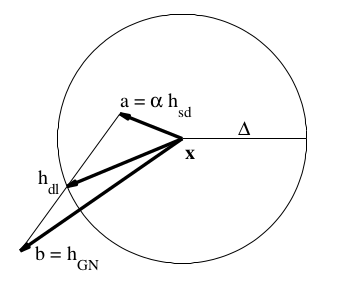
\includegraphics[width=.3\textwidth]{Pictures/dogleg_step.png}
    \caption{信赖域与Dog-Leg法迭代步\citep{tingleff2004methods}}
    \label{fig:dogleg_step}
\end{figure}

\begin{algorithm}[htb!]
\caption{狗腿法}
\begin{algorithmic}
    \State $\Delta \coloneqq \Delta_0, \bm{x} \coloneqq \bm{x}_0$
    \For{$k = 0 \rightarrow k_{max}$}
        \State $k \coloneqq k+1$
        \State 使用式\eqref{eq:lls}计算线性化子问题
        \State 使用式\eqref{eq:gn}计算高斯-牛顿迭代步$\bm{\delta}_{gn}$
        \State 使用式\eqref{eq:sd}计算最速下降迭代步$\bm{\delta}_{sd}$
        \State 使用式\eqref{eq:dl}计算狗腿法步长$\bm{\delta}_{dl}$

        \If{\{步长$\bm{\delta}_{dl}$收敛\}}
            \State 结束优化
        \EndIf

        \State 计算迭代步质量$\varrho$:
        \[
            \varrho = \frac {F(\bm{x})-F(\bm{x}+\bm{\delta}_{dl})}
                            {L(\bm{0})-L(\bm{\delta}_{dl})}
        \]

        \If{\{$\varrho > 0.0$\}}
            \State $\bm{x} \coloneqq \bm{x} + \bm{\delta}_{dl}$
        \EndIf

        \If{\{$\varrho > \epsilon_0$\}}
            \State $\Delta \coloneqq \text{fmax}\{\Delta,3\left\|\bm{\delta}_{dl}\right\|\}$
        \ElsIf{\{$\varrho < \epsilon_1$\}}
            \State $\Delta \coloneqq \Delta/2$
        \EndIf

        \If{\{信赖域$\Delta$收敛\}}
            \State 结束优化
        \EndIf
    \EndFor
\end{algorithmic}
\label{alg:dogleg}
\end{algorithm}


\subsection{舒尔补}\label{sec:schur}

不论是使用高斯-牛顿法,莱文贝格-马夸特方法还是Dog-Leg法,在每一轮迭代过程中,都需要进一步通过求解正规方程这个线性系统来得到每一轮迭代的步长(如 式\eqref{eq:gn},\eqref{eq:lm},\eqref{eq:dl})。根据经验,SLAM问题具有良好的稀疏性:通常三维点状态的数量要远大于相机状态的数量,而且通常三维点之间没有直接联系;同时,只有物理上距离比较接近的三维点状态和相机状态之间有相互约束。因此,由集束调整问题构建的海森矩阵$\mathrm{H}$也具有稀疏的性质,通过对变量适当的排序,将三维点状态和相机状态分别分组,一般可以得到如图~\ref{fig:sparse_matrix}所示的特殊的稀疏结构。

\begin{figure}[htb!]
    \centering
    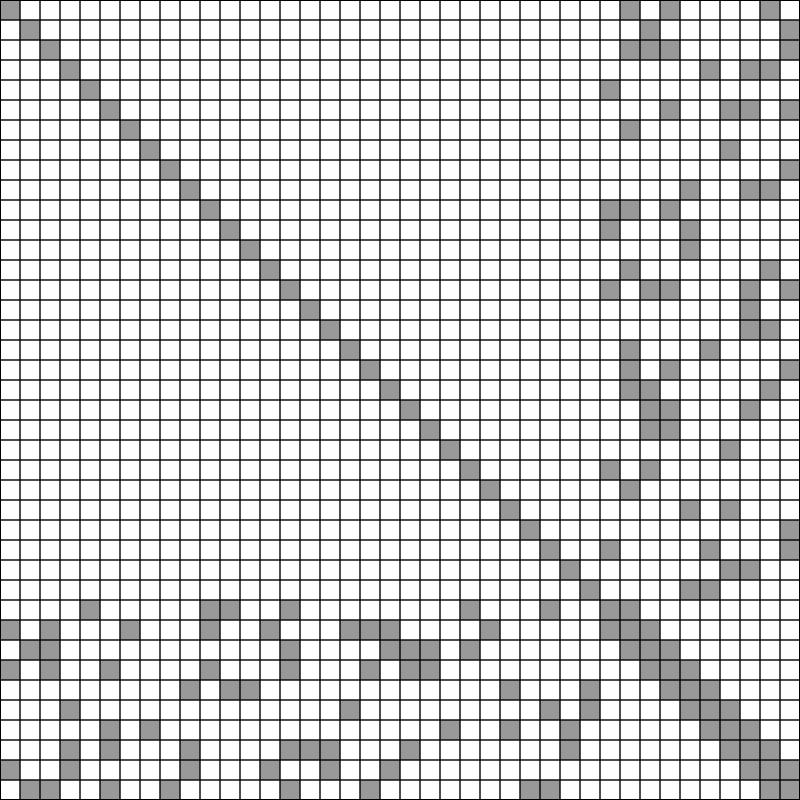
\includegraphics[width=.5\textwidth]{Pictures/sparse_matrix.png}
    \caption{一般的稀疏矩阵结构:左上角部分为三维点状态对应的海森矩阵,呈对角块稀疏状;右下角部分为相机状态对应的海森矩阵,呈条带稀疏状;左下角矩阵为三维点状态和相机状态的相关海森矩阵,只有具有观测关系的三维点和相机之间的相关部分为非零。}
    \label{fig:sparse_matrix}
\end{figure}

对于这样具备特殊稀疏结构的线性系统,可以用舒尔补(Schur complement)来加速求解。舒尔补是一种常用的加速求解稀疏线性系统的方法,特别适用于集束调整问题中的正规方程的求解。其本质上是一种基于高斯消元的分块求解线性系统的方法。首先根据图~\ref{fig:sparse_matrix}对正规方程进行分块:
\begin{equation}
    \mathrm{H} =
    \begin{bmatrix}
        \mathrm{P} & \mathrm{W}^\top \\
        \mathrm{W} & \mathrm{C}
    \end{bmatrix}, \quad
    \bm{\delta} = \begin{bmatrix} \bm{\delta}_p \\ \bm{\delta}_c \end{bmatrix}, \quad
    \bm{\eta} = \begin{bmatrix} \bm{p} \\ \bm{c} \end{bmatrix}
\end{equation}
其中$\mathrm{P}$是三维点状态对应的海森矩阵,$\mathrm{C}$是相机状态对应的海森矩阵,$\mathrm{W}$是三维点状态和相机状态的海森矩阵。求解三维点状态和相机状态之前,先通过行变换构建舒尔补方程:
\begin{equation}
    \left( \mathrm{C}-\mathrm{W}\mathrm{P}^{-1}\mathrm{W}^\top \right)
    \bm{\delta}_c = \bm{c}-\mathrm{W}\mathrm{P}^{-1}\bm{p}
    \label{eq:schur_complement}
\end{equation}

记舒尔补矩阵为$\mathrm{S}\doteq\mathrm{C}-\mathrm{W}\mathrm{P}^{-1}\mathrm{W}^\top$,右侧为$\bm{b}\doteq\bm{c}-\mathrm{W}\mathrm{P}^{-1}\bm{p}$。如前面提到的,集束调整问题中的三维点状态数量远多于相机状态数量,故矩阵$\mathrm{S}$的规模远小于$\mathrm{P}$的规模,通过求解下舒尔补方程:
\begin{equation}
    \bm{\delta}_c = \mathrm{S} \:\setminus\: \bm{b}
    \label{eq:solve_schur}
\end{equation}
可以快速先得到相机状态的迭代步。而又因为矩阵$\mathrm{P}$通常呈块对角状,其逆矩阵的求解$\mathrm{P}^{-1}$也非常容易,通过变量回代又可以高效地求解剩余的三维点状态的迭代步:
\begin{equation}
    \bm{\delta}_p = \mathrm{P}
    \:\setminus\:
    \left( \bm{p}-\mathrm{W}^\top\bm{\delta}_c \right)
    \label{eq:back_sub}
\end{equation}

舒尔补可以加速稀疏线性系统的求解,但需要注意的是,舒尔补一般会造成矩阵的填充效应(fill in)\citep{kaess2008isam},即破坏矩阵稀疏性的情况。在使用舒尔补的时候如果不注意变量的排序,则很容易造成严重的填充。

\subsection{鲁棒估计方法}

最小二乘非常容易受数据中的外点(outliers)影响。也就是说,基于非线性最小二乘的因子图优化对于问题中的错误约束非常敏感。考虑一般的VSLAM,一种常见的产生错误约束的情况就是问题中特征误匹配带来的错误视觉观测约束。错误的约束通常对应着更大的目标函数,为了降低错误约束的影响,通常要引入鲁棒估计的方法(robust estimation)来进一步限制问题。一个带有鲁棒项的非线性最小二乘优化问题(robustified nonlinear least squares)将基本的非线性最小二乘问题\eqref{eq:nls}修改为了如下形式:
\begin{equation}
    R(\bm{x}) = \tfrac{1}{2} \rho(F(\bm{x}))
              = \tfrac{1}{2} \rho \left( \left\| \bm{f}(\bm{x}) \right\|^2 \right)
\label{eq:rnls}
\end{equation}
其中标量函数$\rho(\cdot):\mathbb{R}\mapsto\mathbb{R}$为鲁棒函数(robust function),通常为高度非线性。

由于鲁棒函数$\rho(\cdot)$给原先非线性最小二乘问题又引入了高度的非线性性质,为了保证计算的正确性,求解鲁棒非线性最小二乘问题的时候不能忽略$\rho(\cdot)$二阶导数\citep{triggs1999bundle}:
\begin{equation}
\begin{gathered}
    \mathrm{H} = \mathrm{J}^\top
                 \left(
                     \rho'\mathrm{I} + 2\rho'' \bm{f}(\bm{x}) \bm{f}^\top(\bm{x})
                 \right)
                 \mathrm{J} \\
    \bm{\eta} = -\rho' \mathrm{J}^\top \bm{f}(\bm{x})
\end{gathered}
\label{eq:rnormal_eq}
\end{equation}

可见,鲁棒函数$\rho(\cdot)$会根据每一个目标函数的模其对正规方程的贡献权重,而且随着优化的进行,这个权重会在每一轮迭代中动态地调整。为了达到合理降低外点权重的目标,需要合理选择鲁棒函数形式。由 式\eqref{eq:rnormal_eq}可见,鲁棒函数的选择尽可能地要满足如下几个条件\citep{triggs1999bundle,zhang1995parameter}:
\begin{enumerate}
    \item $\rho(0)=0$
    \item $\rho'(0)=1$
    \item 当$\left\|\bm{f}(\bm{x})\right\|^2$的值处于外点区域时,
          $\rho'(\left\|\bm{f}(\bm{x})\right\|^2)<1$
    \item 当$\left\|\bm{f}(\bm{x})\right\|^2$的值处于外点区域时,
          $\rho''(\left\|\bm{f}(\bm{x})\right\|^2)<0$
\end{enumerate}
其中前两点是为了保证鲁棒函数不对收敛的目标函数造成影响,后两点是为了保证鲁棒函数能有效地降低处于外点的目标函数的权重。常用的鲁棒函数有Cauchy函数:
\begin{equation}
    \rho(s) = \ln(1+s)
\end{equation}
和Huber函数:
\begin{equation}
    \rho(s) =
    \left\{
    \begin{array}{ll}
        s, & s \leq 1 \\
        2\sqrt{s}-1, & s \geq 1
    \end{array}
    \right.
\end{equation}

\begin{figure}[htb!]
    \centering
    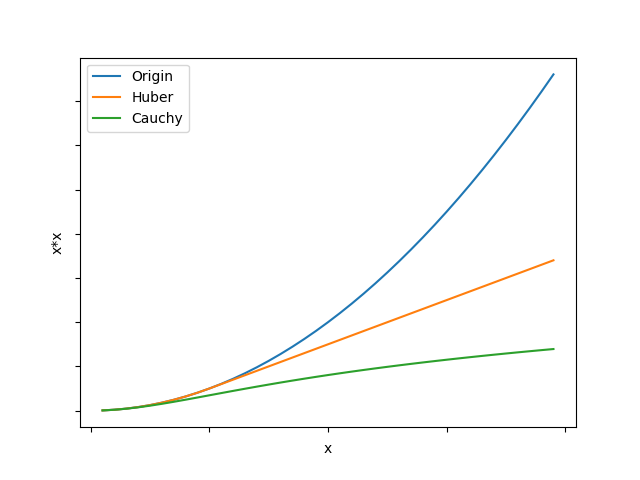
\includegraphics[width=.6\textwidth]{Pictures/robust.png}
    \caption{常用的两种鲁棒函数}
    \label{fig:robust}
\end{figure}

\subsection{边缘状态估计}

对于比较大的系统,状态数量比较多,一般需要通过边缘化对状态进行精简。在图优化中对应的就是通过删减状态节点调整因子图的过程。假设状态$\bm{x}$和$\bm{y}$符合联合高斯分布:
\begin{equation}
p(\bm{x},\bm{y}) \sim \mathcal{N}
\left(
    \begin{bmatrix} \bm{\mu}_x \\ \bm{\mu}_y \end{bmatrix},
    \begin{bmatrix}
        \Sigma_{xx} & \Sigma_{yx}^\top \\
        \Sigma_{yx} & \Sigma_{yy}
    \end{bmatrix}
    \label{eq:joint}
\right)
\end{equation}
对于高斯分布,总是可以使用舒尔补将上面的联合概率分布拆分成两个独立分布的乘积$p(\bm{x},\bm{y})=p(\bm{x}|\bm{y})p(\bm{x})$:
\begin{equation}
\begin{aligned}
    p(\bm{x}|\bm{y}) &\sim \mathcal{N}(
        \bm{\mu}_x+\Sigma_{yx}^\top\Sigma_{yy}^{-1}(\bm{y}-\bm{\mu}_y),
        \Sigma_{xx}-\Sigma_{yx}^\top\Sigma_{yy}^{-1}\Sigma_{yx}) \\
    p(\bm{y}) &\sim \mathcal{N}(\bm{\mu}_y,\Sigma_{yy})
\end{aligned}
\label{eq:indep}
\end{equation}
其中$p(\bm{y})$就是变量$\bm{y}$的边缘概率,而$p(\bm{x}|\bm{y})$则是变量$\bm{x}$关于$\bm{y}$的条件概率。在最小二乘问题中,正规方程的海森矩阵$\mathrm{H}$和右侧$\bm{\eta}$对应的是信息矩阵(information matrix)和信息向量(information vector)\citep{barfoot2017state}。信息矩阵也对应于状态的协方差矩阵的逆$\Sigma^{-1}$,而正规方程的解对应与变量的期望。以状态$\bm{x}$和$\bm{y}$为例,可以构建正规方程:
\begin{equation}
\begin{bmatrix} \bm{x} \\ \bm{y} \end{bmatrix} =
\begin{bmatrix}
    \mathrm{H}_{xx} & \mathrm{H}_{yx}^\top \\
    \mathrm{H}_{yx} & \mathrm{H}_{yy}
\end{bmatrix} \:\setminus\:
\begin{bmatrix} \bm{\eta}_x \\ \bm{\eta}_y \end{bmatrix}
\end{equation}
易得联合概率分布:
\begin{equation}
p(\bm{x},\bm{y}) \sim \mathcal{N}
\left(
\begin{bmatrix}
    \mathrm{H}_{xx} & \mathrm{H}_{yx}^\top \\
    \mathrm{H}_{yx} & \mathrm{H}_{yy}
\end{bmatrix}^{-1}
\begin{bmatrix} \bm{\eta}_x \\ \bm{\eta}_y \end{bmatrix},
\begin{bmatrix}
    \mathrm{H}_{xx} & \mathrm{H}_{yx}^\top \\
    \mathrm{H}_{yx} & \mathrm{H}_{yy}
\end{bmatrix}^{-1}
\right)
\end{equation}
根据 式\eqref{eq:indep},同样使用舒尔补可以计算得到状态$\bm{y}$的边缘概率分布:
\begin{equation}
\begin{gathered}
p(\bm{y}) \sim \mathcal{N}
\Big(
    \overunderbraces{& & \br{1}{\text{边缘信息矩阵}} & & & \br{1}{\text{边缘信息向量}}}
        {
            & ( & \mathrm{H}_{yy}-\mathrm{H}_{yx}\mathrm{H}_{xx}^{-1}\mathrm{H}_{yx}^\top & )^{-1}
            & ( & \bm{\eta}_y-\mathrm{H}_{yx}\mathrm{H}_{xx}^{-1}\bm{\eta}_x              & )
        }
    {& \br{6}{\text{边缘期望}}}
    %
    , \\
    %
    \underbrace{
        (\mathrm{H}_{yy}-\mathrm{H}_{yx}\mathrm{H}_{xx}^{-1}\mathrm{H}_{yx}^\top)^{-1}
    }_{\text{边缘协方差}}
\Big)
\end{gathered}
\end{equation}

如\ref{sec:schur}节中提到的,舒尔补一般会造成稀疏矩阵的填充效应,在使用舒尔补进行边缘化操作的时候,同样会遇到这样的情况。因此,在使用边缘化进行状态删减的时候,也需要注意使用合理的策略选择被删减的状态,尽量减少填充。
